\section{Introduction and Theoretical Framework}

Financial markets exhibit pervasive uncertainty that extends beyond simple volatility measurements. This paper provides a framework for understanding these uncertainties by distinguishing among different types of risk and their implications for market participants. A central question guides our analysis: how can we understand and manage the unexpected in financial markets when the very tools we use to measure risk may be inadequate?

Drawing on both simulated and observed market data, we show how individual stock returns differ sharply from those of diversified portfolios, examine how moral hazard limits diversification in practice and how regulation can mitigate it, and consider why even sophisticated market participants underestimate tail risks.

\subsection{Defining the Unexpected}
Life presents us with countless outcomes we cannot predict with certainty. In financial markets, this uncertainty presents across various dimensions: the outcome of a specific FDA trial, the integrity of corporate management, daily stock market returns, the stability of financial institutions, and especially the beliefs of other market participants.

Mathematically, we represent the range of possible outcomes as a random variable. For any uncertain outcome $X$, we can form an expectation $E[X]$. Something becomes \say{unexpected} to the degree that a realized outcome $x$ deviates from the overall expectation (i.e., when $|x - E[X]|$ is large). Even if a specific outcome is slightly unexpected, it still carries risk, and most won't accept that risk for free.

\subsection{Risk Aversion and the Demand for Compensation}

The foundation of modern finance rests on the assumption that individuals are risk-averse, meaning most require extra compensation if they are taking risk. This stems from the idea of diminishing marginal utility: people derive less additional satisfaction from each incremental unit of consumption or wealth (\autoref{fig:fig1}). Concretely, let $u(w)$ represent an investor’s utility from wealth $w$. We assume $u'(w) > 0$ (utility increases with wealth) but $u''(w) < 0$ (marginal utility decreases), so utility is increasing and concave. 

\begin{figure}[h]
    \centering
    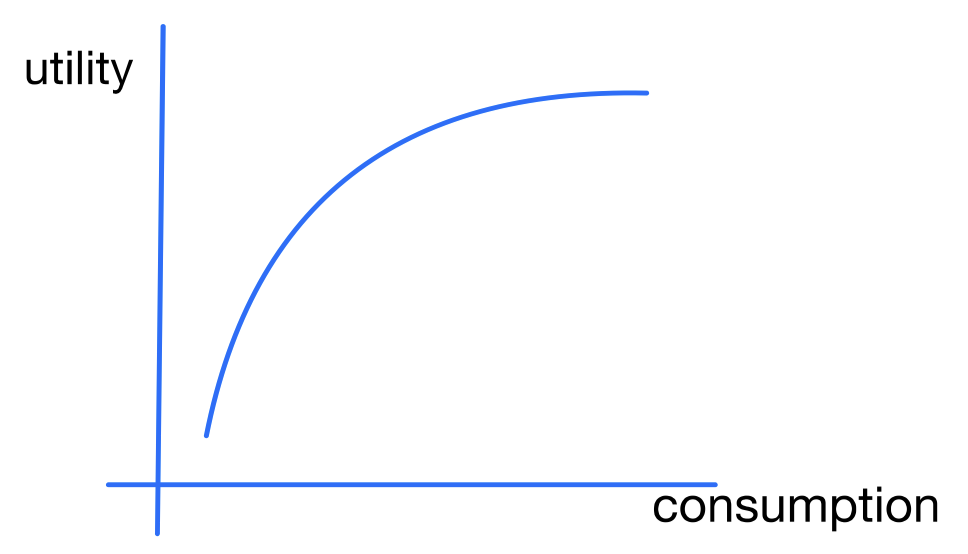
\includegraphics[width=0.50\textwidth]{fig1.png}
    \caption{Concave utility function showing diminishing marginal utility}
    \label{fig:fig1}
\end{figure}

Because of concavity, the average of utilities is less than the utility of the average outcome. Jensen’s inequality formalizes this:
$$E[u(w + \tilde{x})] < u(w + E[\tilde{x}]) = u(w)$$

for a zero-mean ($E[\tilde{x}] = 0$) gamble $\tilde{x}$ (\autoref{fig:fig2}). This inequality implies that the expected utility of a fair gamble is strictly lower than the utility of simply maintaining current wealth $w$. For such a gamble to attract capital, it must offer a positive risk premium $R$ that satisfies:

$$E[u(w \tilde{x})] + R = u(w)$$

\begin{figure}[h]
    \centering
    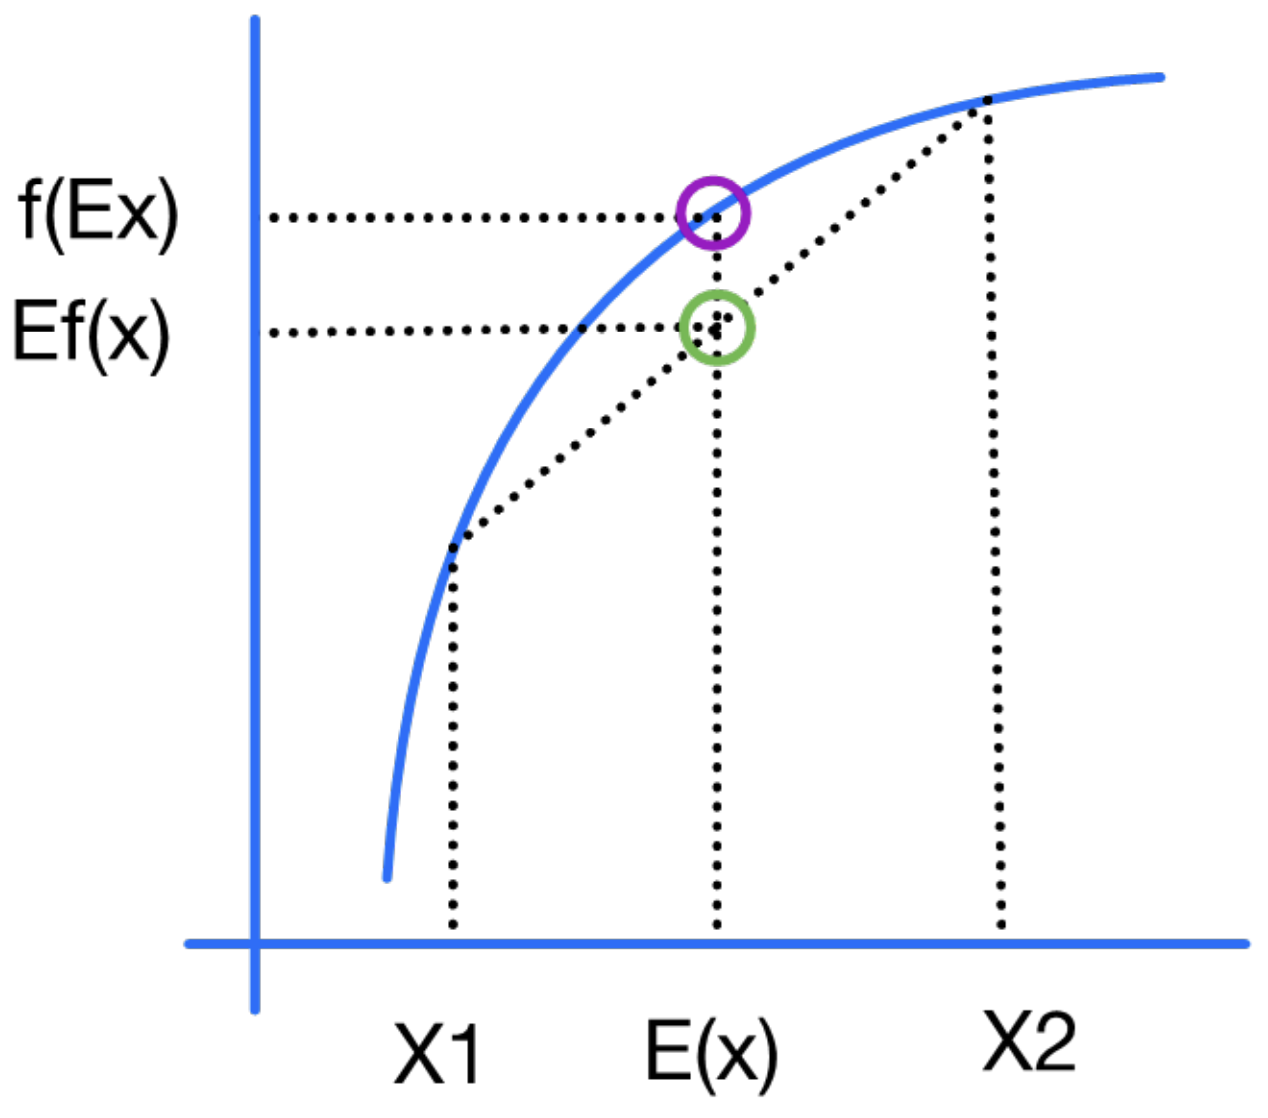
\includegraphics[width=0.50\textwidth]{fig2.png}
    \caption{Jensen's inequality: Expected utility of gamble vs. utility of expected value}
    \label{fig:fig2}
\end{figure}

The size of this risk premium depends on the investor’s risk aversion (the curvature of $u$) and on the distribution of the risky asset’s returns. To understand how large this premium must be in practice, we now turn to the empirical behavior of returns for individual securities and portfolios.